\documentclass[journal,12pt,twocolumn]{IEEEtran}

\usepackage{setspace}
\usepackage{gensymb}

\singlespacing


\usepackage[cmex10]{amsmath}

\usepackage{amsthm}

\usepackage{mathrsfs}
\usepackage{txfonts}
\usepackage{stfloats}
\usepackage{bm}
\usepackage{cite}
\usepackage{cases}
\usepackage{subfig}

\usepackage{longtable}
\usepackage{multirow}

\usepackage{enumitem}
\usepackage{mathtools}
\usepackage{steinmetz}
\usepackage{tikz}
\usepackage{circuitikz}
\usepackage{verbatim}
\usepackage{tfrupee}
\usepackage[breaklinks=true]{hyperref}
\usepackage{graphicx}
\usepackage{graphics}
\usepackage{tkz-euclide}
\usepackage{float}

\usetikzlibrary{calc,math}
\usepackage{listings}
    \usepackage{color}                                            %%
    \usepackage{array}                                            %%
    \usepackage{longtable}                                        %%
    \usepackage{calc}                                             %%
    \usepackage{multirow}                                         %%
    \usepackage{hhline}                                           %%
    \usepackage{ifthen}                                           %%
    \usepackage{lscape}     
\usepackage{multicol}
\usepackage{chngcntr}

\DeclareMathOperator*{\Res}{Res}

\renewcommand\thesection{\arabic{section}}
\renewcommand\thesubsection{\thesection.\arabic{subsection}}
\renewcommand\thesubsubsection{\thesubsection.\arabic{subsubsection}}

\renewcommand\thesectiondis{\arabic{section}}
\renewcommand\thesubsectiondis{\thesectiondis.\arabic{subsection}}
\renewcommand\thesubsubsectiondis{\thesubsectiondis.\arabic{subsubsection}}


\hyphenation{op-tical net-works semi-conduc-tor}
\def\inputGnumericTable{}                                 %%

\lstset{
%language=C,
frame=single, 
breaklines=true,
columns=fullflexible
}
\begin{document}


\newtheorem{theorem}{Theorem}[section]
\newtheorem{problem}{Problem}
\newtheorem{proposition}{Proposition}[section]
\newtheorem{lemma}{Lemma}[section]
\newtheorem{corollary}[theorem]{Corollary}
\newtheorem{example}{Example}[section]
\newtheorem{definition}[problem]{Definition}

\newcommand{\BEQA}{\begin{eqnarray}}
\newcommand{\EEQA}{\end{eqnarray}}
\newcommand{\define}{\stackrel{\triangle}{=}}
\newcommand\hlight[1]{\tikz[overlay, remember picture,baseline=-\the\dimexpr\fontdimen22\textfont2\relax]\node[rectangle,fill=blue!50,rounded corners,fill opacity = 0.2,draw,thick,text opacity =1] {$#1$};}
\bibliographystyle{IEEEtran}
\providecommand{\mbf}{\mathbf}
\providecommand{\pr}[1]{\ensuremath{\Pr\left(#1\right)}}
\providecommand{\qfunc}[1]{\ensuremath{Q\left(#1\right)}}
\providecommand{\sbrak}[1]{\ensuremath{{}\left[#1\right]}}
\providecommand{\lsbrak}[1]{\ensuremath{{}\left[#1\right.}}
\providecommand{\rsbrak}[1]{\ensuremath{{}\left.#1\right]}}
\providecommand{\brak}[1]{\ensuremath{\left(#1\right)}}
\providecommand{\lbrak}[1]{\ensuremath{\left(#1\right.}}
\providecommand{\rbrak}[1]{\ensuremath{\left.#1\right)}}
\providecommand{\cbrak}[1]{\ensuremath{\left\{#1\right\}}}
\providecommand{\lcbrak}[1]{\ensuremath{\left\{#1\right.}}
\providecommand{\rcbrak}[1]{\ensuremath{\left.#1\right\}}}
\theoremstyle{remark}
\newtheorem{rem}{Remark}
\newcommand{\sgn}{\mathop{\mathrm{sgn}}}
\providecommand{\abs}[1]{\left\vert#1\right\vert}
\providecommand{\res}[1]{\Res\displaylimits_{#1}} 
\providecommand{\norm}[1]{\left\lVert#1\right\rVert}
%\providecommand{\norm}[1]{\lVert#1\rVert}
\providecommand{\mtx}[1]{\mathbf{#1}}
\providecommand{\mean}[1]{E\left[ #1 \right]}
\providecommand{\fourier}{\overset{\mathcal{F}}{ \rightleftharpoons}}
%\providecommand{\hilbert}{\overset{\mathcal{H}}{ \rightleftharpoons}}
\providecommand{\system}{\overset{\mathcal{H}}{ \longleftrightarrow}}
	%\newcommand{\solution}[2]{\textbf{Solution:}{#1}}
\newcommand{\solution}{\noindent \textbf{Solution: }}
\newcommand{\cosec}{\,\text{cosec}\,}
\providecommand{\dec}[2]{\ensuremath{\overset{#1}{\underset{#2}{\gtrless}}}}
\newcommand{\myvec}[1]{\ensuremath{\begin{pmatrix}#1\end{pmatrix}}}
\newcommand{\mydet}[1]{\ensuremath{\begin{vmatrix}#1\end{vmatrix}}}
\numberwithin{equation}{subsection}
\makeatletter
\@addtoreset{figure}{problem}
\makeatother
\let\StandardTheFigure\thefigure
\let\vec\mathbf
\renewcommand{\thefigure}{\theproblem}
\def\putbox#1#2#3{\makebox[0in][l]{\makebox[#1][l]{}\raisebox{\baselineskip}[0in][0in]{\raisebox{#2}[0in][0in]{#3}}}}
     \def\rightbox#1{\makebox[0in][r]{#1}}
     \def\centbox#1{\makebox[0in]{#1}}
     \def\topbox#1{\raisebox{-\baselineskip}[0in][0in]{#1}}
     \def\midbox#1{\raisebox{-0.5\baselineskip}[0in][0in]{#1}}
\vspace{3cm}
\title{Assignment 15}
\author{K.A. Raja Babu}
\maketitle
\newpage
\bigskip
\renewcommand{\thefigure}{\theenumi}
\renewcommand{\thetable}{\theenumi}
Download all python codes from 
\begin{lstlisting}
https://github.com/ka-raja-babu/Matrix-Theory/tree/main/Assignment15/Codes
\end{lstlisting}
%
and latex-tikz codes from 
%
\begin{lstlisting}
https://github.com/ka-raja-babu/Matrix-Theory/tree/main/Assignment15
\end{lstlisting}
%
\section{Question No. 2.1(a)(Optimization)}

Find the absolute maximum and absolute minimum value of $f(x)=4x-\frac{1}{2}x^2,x \in \brak{-2,\frac{9}{2}}$ .

\section{Solution}

\begin{lemma}
A function f(x) is said to be convex if following inequality is true for $\lambda \in [0,1] :$  \label{lemma1}
\begin{align}
    \lambda f(x_1) + (1-\lambda)f(x_2) \geq f(\lambda x_1 + (1-\lambda)x_2)
\end{align}
\end{lemma}

Given :
\begin{align}
    f(x) &= 4x-\frac{1}{2}x^2 , x \in \brak{-2,\frac{9}{2}}
\end{align}

Checking convexity of $f(x)$ :
\begin{equation}
\begin{aligned}
    &\lambda\brak{4x_1-\frac{1}{2}x_1^2} + (1-\lambda)\brak{4x_2-\frac{1}{2}x_2^2} \geq \\
    &4\brak{\lambda x_1 + (1-\lambda)x_2} - \frac{1}{2}\brak{\lambda x_1 + (1-\lambda)x_2}^2
\end{aligned}
\end{equation}

resulting in
\begin{align}
    x_1^2\brak{\frac{\lambda^2-\lambda}{2}}+x_2^2\brak{\frac{\lambda^2-\lambda}{2}}+ 2x_1x_2\brak{\frac{\lambda-\lambda^2}{2}} &\geq 0 \\
    \implies \brak{\frac{\lambda^2-\lambda}{2}}\brak{x_1^2+x_2^2-2x_1x_2} &\geq 0 \\
    \implies -\frac{1}{2}\lambda\brak{1-\lambda}\brak{x_1-x_2}^2 &\geq 0 \\
    \implies \frac{1}{2}\lambda\brak{1-\lambda}\brak{x_1-x_2}^2 &\leq 0
\end{align}

Hence,using lemma \ref{lemma1}, given $f(x)$ is a concave function .

\begin{enumerate}
    \item For Maxima : \\
    Using gradient ascent method,
    \begin{align}
        x_{n+1} &= x_n + \alpha \nabla f(x_n) \\
        \implies x_{n+1} &= x_n + \alpha \brak{4-x}
    \end{align}
    
    Taking $x_0=-2,\alpha=0.001$ and precision= \\ 0.00000001,values obtained using python are:
    \begin{align}
        \boxed{\text{Maxima} = 7.999999999950196 \approx 8 }\\
        \boxed{\text{Maxima Point} = 3.9999900196756437 \approx 4}
    \end{align}
    
    \numberwithin{figure}{section}
    \begin{figure}[!ht]
    \centering
    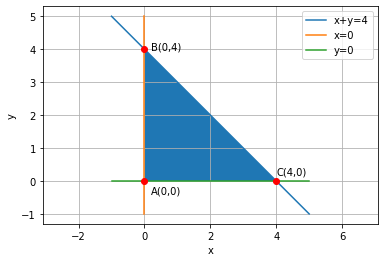
\includegraphics[width=\columnwidth]{Figure15}
    \caption{$f(x)=4x-0.5x^2$}
    \label{f(x)}	
    \end{figure}

    \item For Minima : \\
    
    \numberwithin{table}{section}
    \begin{table}[!ht]
    \centering
    \begin{tabular}{|c|c|} 
    \hline
    $x$ & $f(x)$ \\
    \hline
    -2 & -10 \\
    \hline
    4 & 8 \\
    \hline
    4.5 & 7.875 \\
    \hline
    \end{tabular}
    \caption{Value of $f(x)$}
    \label{tab:table1}
    \end{table}
    
    Critical point is given by
    \begin{align}
        \nabla f(x) &= 0 \\
        \implies x &= 4
    \end{align}
    
    and,end points are $x=-2$ and $x=4.5$ .
    
    Using table \ref{tab:table1},
    \begin{align}
        \boxed{\text{Minima} = -10}\\
        \boxed{\text{Minima Point} = -2}
    \end{align}
    
\end{enumerate}

\end{document}

